%%%%%%%%%%%%%%%%%%%%%%%%%%%%%%%%%%%%%%%%%%%%%%%%%%%%%%
% A Beamer template for Ritsumeikan University       %
% Author: Ming-Hao Xu (Xu Minghao)                   %
% Date:   April 2022.                                %
% LPPL Licensed.                                     %
%%%%%%%%%%%%%%%%%%%%%%%%%%%%%%%%%%%%%%%%%%%%%%%%%%%%%%

\documentclass{beamer}
\usepackage{hyperref}

\usepackage[UTF8]{ctex}
\usepackage[T1]{fontenc}

% other packages
\usepackage{latexsym,amsmath,xcolor,multicol,booktabs,calligra}
\usepackage{graphicx,pstricks,listings,stackengine}
\usefonttheme[onlymath]{serif}

% dummy text; remove it when working on this template
\usepackage{lipsum}

\author{Ebola}
\title{高级字符串算法:后缀自动机、后缀数组、回文自动机}
\institute{
    Institute of Mathematics, \\
    Zhejiang University.
}
\date{July, 2023}
\usepackage{Ritsumeikan}

% defs
\def\cmd#1{\texttt{\color{red}\footnotesize $\backslash$#1}}
\def\env#1{\texttt{\color{blue}\footnotesize #1}}
\definecolor{deepblue}{rgb}{0,0,0.5}
\definecolor{deepred}{rgb}{0.6,0,0}
\definecolor{deepgreen}{rgb}{0,0.5,0}
\definecolor{halfgray}{gray}{0.55}

\lstset{
    basicstyle=\ttfamily\tiny,
    keywordstyle=\bfseries\color{deepblue},
    emphstyle=\ttfamily\color{deepred},    % Custom highlighting style
    stringstyle=\color{deepgreen},
    numbers=left,
    numberstyle=\small\color{halfgray},
    rulesepcolor=\color{red!20!green!20!blue!20},
    frame=shadowbox,
}


\begin{document}

\begin{frame}
    \titlepage
\end{frame}

\begin{frame}
    \tableofcontents[sectionstyle=show,subsectionstyle=show/shaded/hide,subsubsectionstyle=show/shaded/hide]
\end{frame}

\section{后缀自动机}

\begin{frame}{模板题}
    \small
    给定一个只包含小写字母的字符串$S$,求$S$的所有出现次数不为$1$的子串的出现次数乘上该子串长度的最大值。$|S|\leq 10^6$
\end{frame}

\begin{frame}{什么是SAM}
    \small
    后缀自动机(SAM)是一种特殊的有限状态自动机(DFA),它符合以下性质:

    \begin{itemize}
        \item 转移图是有向无环图,且每个转移接受且只接受一个字符
        \item 接受且只接受$S$的所有后缀
        \item 在符合以上性质的基础上,节点数最少
    \end{itemize}
    
    如果只考虑前两条,其实只要把$S$的所有后缀插入字典树即可,节点数有$O(n^2)$个。
\end{frame}

\begin{frame}[fragile]{代码}
    \begin{minipage}{\linewidth}
    \begin{lstlisting}[language=c++]
        void insert(int c)
        {
            int p=lst,np=++tot;len[np]=len[p]+1;
            while(p&&!ch[p][c]) ch[p][c]=np,p=prt[p];
            if(!p) prt[np]=1;
            else
            {
                int q=ch[p][c];
                if(len[p]+1==len[q]) prt[np]=q;
                else
                {
                    int nq=++tot;len[nq]=len[p]+1;
                    memcpy(ch[nq],ch[q],sizeof(ch[nq]));
                    prt[nq]=prt[q];prt[q]=prt[np]=nq;
                    while(ch[p][c]==q) ch[p][c]=nq,p=prt[p];
                }
            }
            sz[np]=1;lst=np;
        }
    \end{lstlisting}
    \end{minipage}

    这是SAM的核心代码,很短。
\end{frame}

\begin{frame}{endpos等价类}
    \small
    我们首先提出endpos等价类这个概念。$endpos(P)$表示模式串$P$在$S$中所有出现的结束位置的集合,那么$endpos$相同的模式串就可以共用一个节点。例如串"aababc"中,"b"和"ab"的endpos都是$\{3,5\}$,说明他们总是一起出现,所以可以共用一个节点。我们把$endpos$相同的模式串组成的集合称为一个$endpos$ \textbf{等价类}。

    \pause \vspace{1em}
    显然,对于一个等价类内的两个模式串$P_1$和$P_2$,如果$|P_1|<|P_2|$,那么$P_1$一定是$P_2$的后缀,因此,在一个等价类中,一定存在一个\textbf{最长}的字符串$P$,等价类中的所有字符串都是$P$的后缀。

    \pause \vspace{1em}
    根据位于$P$ \textbf{前面的那一个字符}是什么,可以把原等价类划分为若干个等价类。例如在"aababc"中,我们已经知道"ab"出现了两次,但首次出现时前面的那一个字符是"a",再次出现时前面那个字符是"b",而"aab"与"bab"属于两个不同的等价类,因此我们可以把等价类$\{3,5\}$划分成$\{3\}$和$\{5\}$
\end{frame}

\begin{frame}{endpos等价类}
    \small
    我们可以认为,空串的$endpos$等价类是$\{1,...,n\}$,而所有等价类都是由此一步一步划分来的,形成一个树的结构,总节点数不会超过$2n-1$

    \begin{figure}[H]
        \centering
        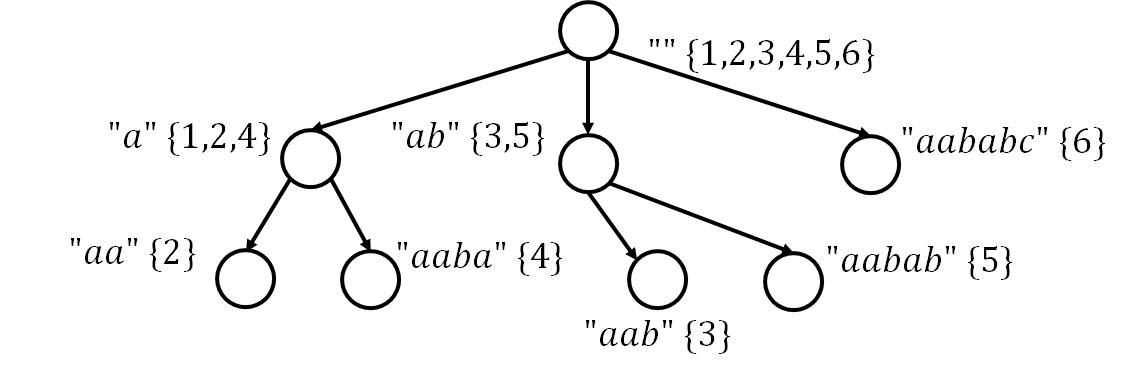
\includegraphics[width=0.7\textwidth]{pic/parent.png}
    \end{figure}

    这棵树就是parent树,他的节点和SAM的状态一一对应。注意,划分过程中可能会丢失元素,例如图中"a"第一个出现的位置前面没有字符,所以划分后会丢失一个元素,这一点在做dp的时候很关键。
\end{frame}

\begin{frame}{构造SAM}
    \small
采取动态构造的方法,一个一个地把字符加进去。考虑向一个已知的字符串的后面添加一个字符,它的SAM会如何变化。

\pause \vspace{1em}
设 go[st][ch] 表示状态st接受字符ch后转移到的状态,fa[st]为该状态在parent树上的父节点,len[st]为该状态对应的$endpos$等价类中最长串的长度,last为加入新字符前整个字符串所在的等价类对应的状态。

\pause \vspace{1em}
一个基本的观察是:从last开始在parent树上往上爬,一定能遍历加入新字符前所有后缀的对应节点。加入一个新的字符,其实就是给之前部分后缀新增了转移。

\pause \vspace{1em}
所以当新增字符ch时,我们创建一个新状态cur(其中len[cur]=len[last]+1),然后从last开始往上爬,对于遇到的每个状态p,如果p还不能通过ch转移,那我们就新增一个转移go[p][ch]=cur,然后继续往上爬,直到某个p可以通过ch转移到状态q ,或者处理完根节点为止。这分为三种情况
\end{frame}

\begin{frame}{第一种情况}
    \small
    \textbf{没有找到要找的q}。这只可能出现在加入了从未加入过的字符的时候,此时直接令fa[cur]为根节点然后退出即可。 (当然退出后还需要把last设为cur,这对三种情况都是一样的)
    
    \begin{figure}[H]
        \centering
        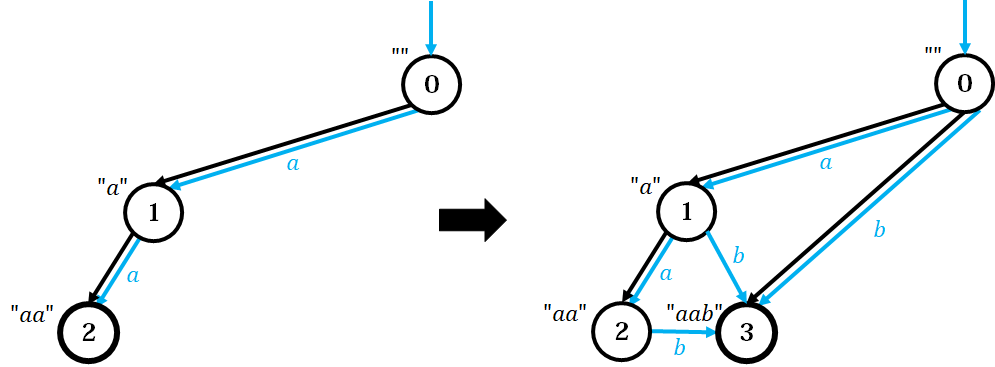
\includegraphics[width=0.9\textwidth]{pic/case1.png}
    \end{figure}
\end{frame}

\begin{frame}{第二种情况}
    \small
    找到了$q$,且len[p]+1==len[q]。这种情况下我们直接令fa[cur]=q然后退出即可。这是因为$p$所对应集合中每个字符串在后面加上一个$ch$都能构成一个$q$对应集合的字符串,而$p$对应集合都是原字符串的后缀,所以$q$对应集合都是新字符串的后缀,应作为$cur$的父亲节点。

    \begin{figure}[H]
        \centering
        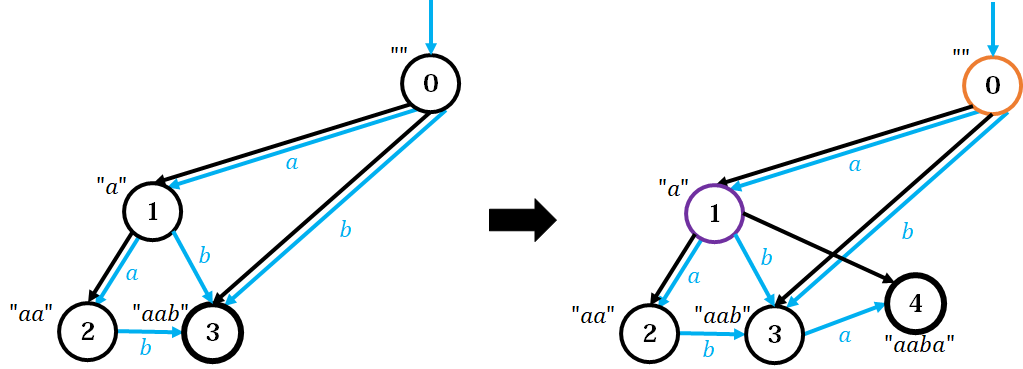
\includegraphics[width=0.9\textwidth]{pic/case2.png}
    \end{figure}
\end{frame}

\begin{frame}{第三种情况}
    \small
    找到了$q$,但len[p]+1$\neq$len[q]。我们新建一个$r$节点,它拥有$q$节点的所有出边,且fa也与$q$节点相同,但是len[r]=len[p]+1。我们从$p$节点继续往上爬,把所有接受$ch$而到达$q$的转移的目标改为$r$(注意只要有一个节点不能接受$ch$那它的祖先都不能接受$ch$,要及时退出循环)。最后令fa[cur]=fa[q]=r。
    
    \begin{figure}[H]
        \centering
        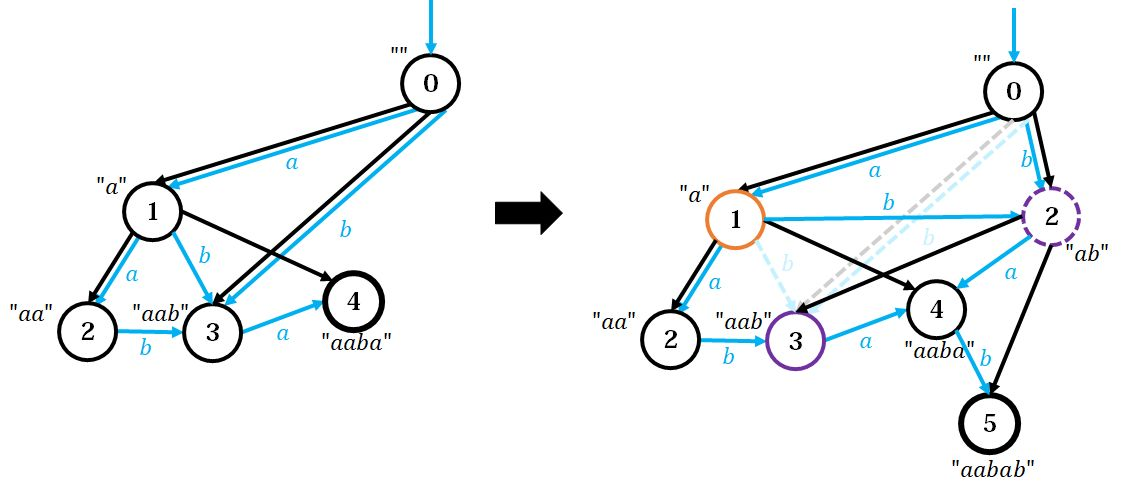
\includegraphics[width=0.8\textwidth]{pic/case3.jpg}
    \end{figure}

    \pause 这里和第二种情况有本质区别,因为$q$不仅仅包含新字符串的后缀,比如下图中3号点除了"ab"还包含了"aab",我们不得不将它拆分开。
\end{frame}

\begin{frame}{一个SAM的例子}
    \small
    下图是字符串"aababb"构成的SAM

    \begin{figure}[H]
        \centering
        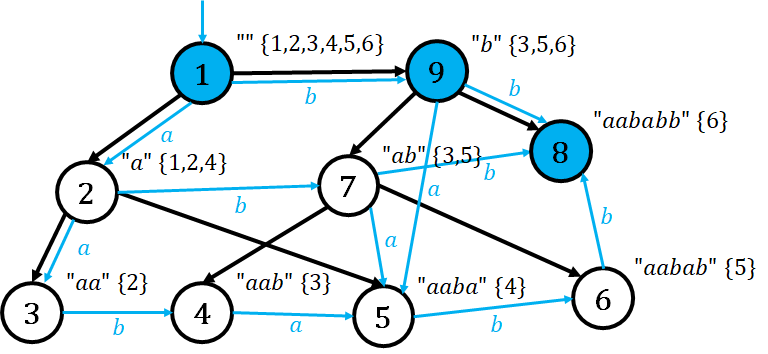
\includegraphics[width=0.8\textwidth]{pic/sameg.png}
    \end{figure}

    复杂度:总状态数不超过$2n-1$,总转移数不超过$3n-4$,构建SAM的复杂度为$O(mn)$,其中$m$为字符集大小。证明见OIwiki
\end{frame}

\begin{frame}{例题选讲}
    \small
    求模式串$P$是不是字符串$S$的子串。

    \pause 【解】建S的SAM,把P放进去跑即可。
\end{frame}

\begin{frame}{例题选讲}
    \small
    求模式串$P$在字符串$S$中的出现次数。

    \pause \vspace{1em}
    【解】建S的SAM,其实就是求$p$对应节点的$endpos$集合的大小,在parent树上dp。

    \pause \vspace{1em}
    对于划分后丢失元素的节点(他所代表的串是$S$的前缀),dp值为子节点dp值之和再加一,其余点则无需加一。其实只要在建SAM的时候让dp[cur]=1即可。

    \pause \vspace{1em}
    小技巧:在parent树上dp的时候不需要dfs,只要把节点按len做一个桶排,然后从大到小枚举,就等价于在parent树上自底向上dp。
\end{frame}

\begin{frame}{例题选讲}
    \small
    求字符串$S$本质不同的子串个数。

    \pause \vspace{1em}
    【解】建S的SAM,从parent树的角度考虑,每个节点代表了len[p]-len[fa[p]]个子串(因为长度不同,自然互不相同)。另外由parent树的划分意义,不同节点代表的子串一定都不同,且任何一个子串必然被parent树上某一点代表。累加该值即可。
\end{frame}

\begin{frame}[fragile]{例题选讲:SPOJ 1811}
    \small
    求字符串$S$与$T$的最长公共子串。

    \pause \vspace{1em}
    【解】建S的SAM,对$T$的每个前缀,求他在$S$中出现过的最长后缀。其实就是把T放进去跑,一直到跑不动了就跳到parent树上的父节点继续跑,跳parent的时候要维护当前最长后缀的长度。

    \pause \vspace{.5em}
    \begin{lstlisting}[language=c++]
    int lcs(char *s)
    {
        int m=strlen(s), l=0, p=1, ans=0;
        for(int i=0;i<m;i++)
        {
            int c=s[i]-'a';
            while(p!=1 && go[p][c]==0)
                p=fa[p], l=len[p]; //维护当前最长后缀长度
            if(go[p][c]) p=go[p][c], l++;
            ans=max(ans,l);
        }
        return ans;
    }
    \end{lstlisting}
\end{frame}

\begin{frame}{例题选讲:(UVA 719) (P1368) 最小表示法}
    \small
    有N组数据,每组给你一串字符串,但是这串字符串是环形的,让你找个位置切开,使得它的字典序最小,输出切开的位置(如果答案不唯一,输出最小位置)

    \pause \vspace{1em}
    【解】遇到循环串的问题一般都先把串复制一遍得到SS,建SS的SAM。

    \pause \vspace{1em}
    SS的SAM能且仅能接受SS的所有子串,所以从根节点出发跑$|S|$步得到的就是$S$的某个循环排列,一直沿最小字典序的转移边跑即可。
\end{frame}

\begin{frame}{例题选讲:UVA 719}
    \small
    给出一个字符串$S$,长度不超过$90000$。询问$q$次,每次给一个$k$,求所有本质不同的子串中,字典序第$k$小的。

    \pause \vspace{1em}
    【解】先建$S$的SAM,求出$size[p]$表示从$p$出发能跑出几个子串,逆拓扑序dp即可。

    \pause \vspace{1em}
    对于一个询问,从根节点出发,每次从小到大枚举字母$ch$,如果$size[go[cur][ch]]\geq k$,就往$ch$走;否则$k=k-size[go[cur][ch]]$,继续枚举$ch$
\end{frame}

\begin{frame}{例题选讲:LNOI2022 串}
    \small
多组数据,每次给定一个英文小写字母构成的字符串 $S$,你需要找到一个尽可能长的字符串序列 $(T_0, T_1, \ldots, T_l)$,满足:

\begin{itemize}
\item $T_0$ 是 $S$ 的子串;
\item $\forall 1 \le i \le l$,$\lvert T_i \rvert - \lvert T_{i - 1} \rvert = 1$;
\item $\forall 1 \le i \le l$,存在 $S$ 的一个长度为 $\lvert T_i \rvert + 1$ 的子串 $S'_i$,使得 $S'_i$ 的长度为 $\lvert T_{i - 1} \rvert$ 的前缀为 $T_{i - 1}$,长度为 $\lvert T_i \rvert$ 的后缀为 $T_i$。
\end{itemize}

输出这样的字符串序列的长度的最大值(即 $l$ 的最大值)。

\vspace{1em}

设 $\sum |S|$ 表示测试点中所有测试数据的字符串长度和。对于 $100 \%$ 的测试数据,$1 \le \lvert S \rvert \le 5 \times {10}^5$,$1 \le \sum \lvert S \rvert \le 1.5 \times {10}^6$。

\end{frame}

\begin{frame}{例题选讲:LNOI2022 串}
    \small
    【题解】观察条件:
    \begin{itemize}
        \item $T_0$ 是 $S$ 的子串;
        \item $\forall 1 \le i \le l$,$\lvert T_i \rvert - \lvert T_{i - 1} \rvert = 1$;
        \item $\forall 1 \le i \le l$,存在 $S$ 的一个长度为 $\lvert T_i \rvert + 1$ 的子串 $S'_i$,使得 $S'_i$ 的长度为 $\lvert T_{i - 1} \rvert$ 的前缀为 $T_{i - 1}$,长度为 $\lvert T_i \rvert$ 的后缀为 $T_i$。
    \end{itemize}

    用$[i,j]$表示子串$S[i...j]$,我们构造一个序列$[i,j]\to [i-1,j-2]\to [i-2,j-4]...$,一直这样下去直到长度为$0$或到头了,得到一列子串,把它倒过来,就符合上面的条件。所以答案显然至少为$\left\lfloor\frac{n}{2}\right\rfloor$。

    \pause \vspace{1em}
    现在考虑正向过程。我们从$T_0=\varnothing$开始,每次左端点往右移一个,同时长度加一。如果想要答案更大,一定要有一个左端点回跳的过程。如果现在位于$[l_2,r_2]$,前面恰好有一个$[l_1,r_1]$和$[l_2,r_2]$是一样的,就可以跳回前面。
\end{frame}

\begin{frame}{例题选讲:LNOI2022 串}
    \small
    枚举最后一次回跳。那么我们现在的过程就是,挑选某一个出现至少两次的子串,设位置分别为$[l_1,r_1]$和$[l_2,r_2]$,从空集开始构造到$[l_2,r_2]$,然后回跳到$[l_1,r_1]$,接下来一直向右构造到底。答案就是
    \begin{equation*}
        r_1-l_1+1+\left\lfloor\frac{n-r_1}{2}\right\rfloor
    \end{equation*}

    \pause \vspace{1em}
    还有一个问题:怎么确保能从空串一直构造到$[l_2,r_2]$?

    \pause \vspace{1em}
    可以从$[l_2,r_2]$开始,向左反向构造,到了$[l_1,r_1]$内就跳回到$[l_2,r_2]$中,再继续向左反向构造。

    \pause \vspace{1em}
    需要SAM。对于一个节点(一个$endpos$等价类),你需要知道他表示的最长串出现了多少次(这需要自底向上dp累加)、第一个$endpos$(这需要自底向上dp取min)、这个等价类中最长的串长(也就是len),然后按上式算答案取最大值即可。
\end{frame}

\section{后缀数组}

\begin{frame}{问题引入}
    \small
    给定字符串$S$,$|S|=n$,求$S$排名为1,2,...,n的后缀的起始位置。
\end{frame}

\begin{frame}[fragile]{基本数组}
    \small
    \begin{itemize}
        \item \verb|sa[i]|:排名为$i$的后缀的起始位置
        \item \verb|rk[i]|:起始位置为$i$的后缀的排名
    \end{itemize}
\end{frame}

\begin{frame}{倍增法}
    \small
    \begin{figure}[H]
        \centering
        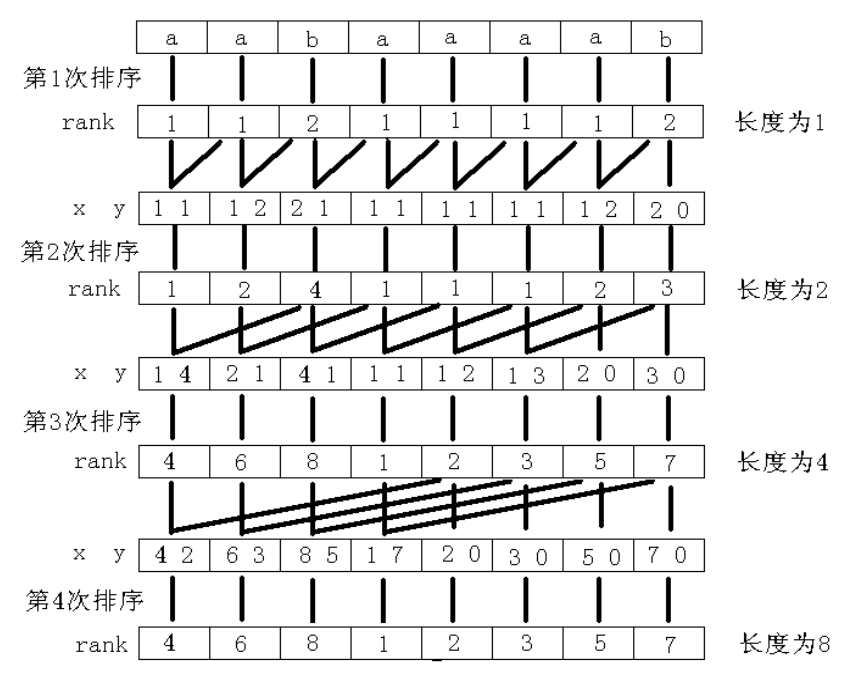
\includegraphics[width=.8\textwidth]{pic/sa2.png}
    \end{figure}
\end{frame}

\begin{frame}[fragile]{倍增法}
    \small
    \begin{itemize}
        \item \verb|rk[i]|的初值是\verb|s[i]|
        \pause \item 对(\verb|rk[i]|,\verb|rk[i+1]|)排序,可以得到从每个$i$开始的长为$2$的子串(长度不足$2$的末尾补空字符)的排名,将结果更新到\verb|rk[i]|
        \pause \item 对(\verb|rk[i]|,\verb|rk[i+2]|)排序,可以得到从每个$i$开始的长为$4$的子串(长度不足$4$的末尾补空字符)的排名,将结果更新到\verb|rk[i]|
        \item ……
    \end{itemize}

    \pause
    如果每一步的排序用\verb|sort|,就得到了$O(n\log^2 n)$的做法。
\end{frame}

\begin{frame}[fragile]{朴素倍增法}
    \small
    \begin{lstlisting}[language=c++]
  for (i = 1; i <= n; ++i) sa[i] = i, rk[i] = s[i];
  for (w = 1; w < n; w <<= 1) {
    sort(sa + 1, sa + n + 1, [](int x, int y) {
      return rk[x] == rk[y] ? rk[x + w] < rk[y + w] : rk[x] < rk[y];
    });  // 这里用到了 lambda
    memcpy(oldrk, rk, sizeof(rk));
    // 由于计算 rk 的时候原来的 rk 会被覆盖,要先复制一份
    for (p = 0, i = 1; i <= n; ++i) {
      if (oldrk[sa[i]] == oldrk[sa[i - 1]] &&
          oldrk[sa[i] + w] == oldrk[sa[i - 1] + w]) {
        rk[sa[i]] = p;
      } else {
        rk[sa[i]] = ++p;
      }  // 若两个子串相同,它们对应的 rk 也需要相同,所以要去重
    }
  }
    \end{lstlisting}
\end{frame}

\begin{frame}[fragile]{双关键字基数排序}
    \small
    注意到对(\verb|rk[i]|,\verb|rk[i+w]|)排序时,关键字的值域是$0,...,n$,所以可以用基数排序来做这个双关键字排序。(基数排序是对相同关键字是保原序的,所以先排第二关键字,然后再排第一关键字)
    \begin{lstlisting}[language=c++]
    // 对第二关键字:id[i] + w进行计数排序
    memset(cnt, 0, sizeof(cnt));
    memcpy(id + 1, sa + 1, n * sizeof(int));
    for (i = 1; i <= n; ++i) ++cnt[rk[id[i] + w]];
    for (i = 1; i <= m; ++i) cnt[i] += cnt[i - 1];
    for (i = n; i >= 1; --i) sa[cnt[rk[id[i] + w]]--] = id[i];

    // 对第一关键字:id[i]进行计数排序
    memset(cnt, 0, sizeof(cnt));
    memcpy(id + 1, sa + 1, n * sizeof(int));
    for (i = 1; i <= n; ++i) ++cnt[rk[id[i]]];
    for (i = 1; i <= m; ++i) cnt[i] += cnt[i - 1];
    for (i = n; i >= 1; --i) sa[cnt[rk[id[i]]]--] = id[i];
    \end{lstlisting}
\end{frame}

\begin{frame}[fragile]{常数优化}
    上面的代码复杂度为$O(n\log n)$,常数大约为$7$,可以进一步把常数优化到$5$。
    \vspace{1em}
    第二关键字排序的实质,其实就是把超出字符串范围(即 \verb|sa[i]+w>n|)的 \verb|sa[i]| 放到 \verb|sa| 数组头部,然后把剩下的依原顺序放入,所以第二关键字的排序可以写为:
    \begin{lstlisting}[language=c++]
    for (p = 0, i = n; i > n - w; --i) id[++p] = i;
    for (i = 1; i <= n; ++i) {
        if (sa[i] > w) id[++p] = sa[i] - w;
    }
    \end{lstlisting}
\end{frame}

\begin{frame}[fragile]{完整代码}
    \small
    \begin{lstlisting}[language=c++]
m = 130;
for(int i=1;i<=n;i++) c[rk[i]=s[i]]++;
for(int i=1;i<m;i++) c[i+1]+=c[i];
for(int i=n;i>=1;i--) sa[c[rk[i]]--]=i;
for(int k=1;k<=n;k<<=1)
{
    int num=0;
    for(int i=n-k+1;i<=n;i++) y[++num]=i;
    for(int i=1;i<=n;i++) if(sa[i]>k) y[++num]=sa[i]-k;
    for(int i=1;i<=m;i++) c[i]=0;
    for(int i=1;i<=n;i++) tmp[i]=rk[y[i]];
    for(int i=1;i<=n;i++) c[tmp[i]]++;
    for(int i=1;i<m;i++) c[i+1]+=c[i];
    for(int i=n;i>=1;i--) sa[c[tmp[i]]--]=y[i];
    num=1;swap(rk,y);rk[sa[1]]=1;
    for(int i=2;i<=n;i++)
        rk[sa[i]]=(y[sa[i]]!=y[sa[i-1]]||y[sa[i]+k]!=y[sa[i-1]+k])?++num:num;
    if(num==n) break;
    m=num;
}
    \end{lstlisting}
\end{frame}

\begin{frame}{例题选讲:「USACO07DEC」Best Cow Line}
给你一个字符串,长度不超过$5\times 10^5$,每次从首或尾取一个字符组成字符串,问所有能够组成的字符串中字典序最小的一个。

\vspace{1em}\pause
【题解】枚举选头还是选尾,把反串接在正串后面,中间用一个ASCII码很大的分隔符隔开,借助后缀数组$O(1)$判断即可。
\end{frame}

\begin{frame}[fragile]{height数组}
    要想让SA变得更有用,我们还需要height数组:

    \verb|height[i]=LCP(sa[i],sa[i-1])|,特别地,\verb|height[1]=0|

    \vspace{1em}
    符号\verb|LCP(i,j)|表示字符串S从$i$开始的后缀与从$j$开始的后缀的最长公共前缀长度
\end{frame}

\begin{frame}[fragile]{构建height数组}
    我们有性质:\verb|height[rk[i]] >= height[rk[i-1]]-1|

    \pause \vspace{1em} 暴力求即可。
    \begin{lstlisting}[language=c++]
for (i = 1, k = 0; i <= n; ++i) {
    if (rk[i] == 0) continue;
    if (k) --k;
    while (s[i + k] == s[sa[rk[i] - 1] + k]) ++k;
    height[rk[i]] = k;
}
    \end{lstlisting}
\end{frame}

\begin{frame}[fragile]{构建height数组}
    \small
    证明性质:\verb|height[rk[i]] >= height[rk[i-1]]-1|

    \pause \vspace{1em}
    【证】当 \verb|height[rk[i-1]] <= 1|时,显然成立,现在设\verb|height[rk[i-1]] > 1|。

    由定义,\verb|height[rk[i-1]]=LCP(i-1,sa[rk[i-1]-1])|,记:

    \verb|[i-1,n]=aAD|,\verb|[sa[rk[i-1]-1],n]=aAB|,其中\verb|a|是字母,\verb|A,B,D|都是字符串,从排名来看应该有\verb|B<D|,另外:

    \verb|[i,n]=AD|,\verb|[sa[rk[i-1]-1]+1,n]=AB|

    由定义,\verb|height[rk[i]]=LCP(i,sa[rk[i]-1])|,因此根据排名,有

    \verb|AB <= [sa[rk[i]-1],n] <= AD|

    所以\verb|[sa[rk[i]-1],n]=AC|,因此\verb|height[rk[i]] >= |A||,证毕。
\end{frame}

\begin{frame}[fragile]{例题选讲}
    \small
    给定一个字符串,求两个子串\verb|[a,m]|和\verb|[b,p]|的最长公共前缀,多组询问。

    \vspace{1em}\pause

    【题解】性质:\verb|LCP(sa[i],sa[j])=min(height[i+1],height[i+2],...,height[j])|

    \vspace{1em}\pause
    令\verb|i=rk[a]|,\verb|j=rk[b]|,对\verb|height|数组做RMQ即可。若\verb|LCP(sa[i],sa[j])|超过了\verb|min(m-a,p-b)+1|,那么答案应该是后者。
\end{frame}

\begin{frame}[fragile]{例题选讲:「USACO06DEC」Milk Patterns}
\small
给定字符串S,求出现至少 $k$ 次的子串的最大长度

\vspace{1em}\pause
【题解】出现至少 $k$ 次意味着后缀排序后有至少连续 $k$ 个后缀以这个子串作为公共前缀。

\vspace{1em}\pause
所以,求出每相邻 $k-1$ 个 $height$ 的最小值,再求这些最小值的最大值就是答案。

\vspace{1em}\pause
做滑动窗口即可,可以单调队列,也可以set
\end{frame}

\begin{frame}[fragile]{例题选讲:Distinct Substrings}
\small
给定一个字符串,求该字符串含有的本质不同的子串数量

\vspace{1em}\pause
【题解】子串就是后缀的前缀,所以可以枚举每个后缀,计算前缀总数,再减掉重复。前缀总数其实就是子串个数,为 $n(n+1)/2$。

\vspace{1em}\pause
如果按后缀排序的顺序枚举后缀,每次新增的子串就是除了与上一个后缀的 LCP 剩下的前缀。这些前缀一定是新增的,且只有这些前缀是新增的。

\vspace{1em}\pause
所以答案为:
\begin{equation*}
    \frac{n(n-1)}{2}-\sum_{i=2}^n height[i]
\end{equation*}
\end{frame}

\begin{frame}[fragile]{例题选讲:Musical Themes}
\small
给定一个字符串,求长度至少为$4$且不重叠出现至少两次的最长子串
\vspace{1em}

字符集88,串长$10^5$(洛谷那个题只有5000,我们加强一下)

\vspace{1em}
本题历史地位:楼教主男人八题、2009年集训队论文例题
\end{frame}

\begin{frame}[fragile]{例题选讲:Musical Themes}
\small
【题解】二分答案,转化为判定是否存在长度至少为$4$且不重叠出现至少两次的长为$k$的子串。

\vspace{1em}\pause
对排好序的后缀分组,使得每一个组内所有后缀的最长公共前缀都不小于$k$,借助height数组即可实现这个分组。例如字符串“aabaaaab”在$k=2$时的后缀分组:
\begin{figure}[H]
    \centering
    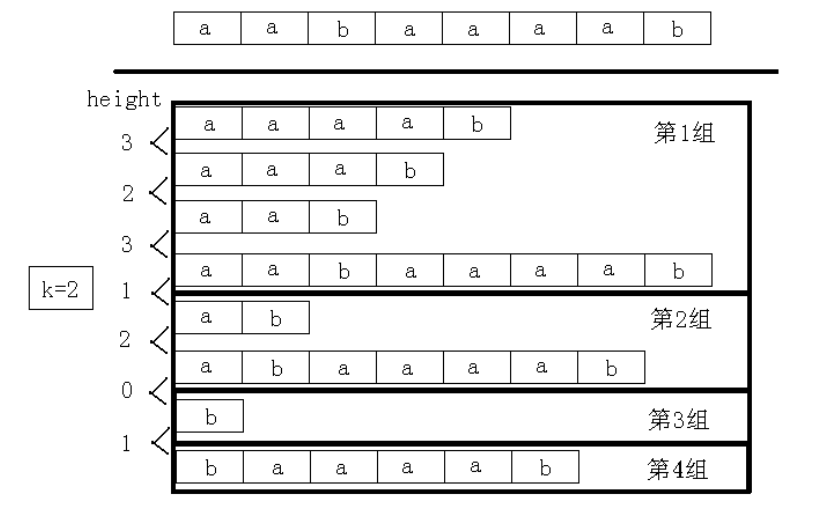
\includegraphics[width=0.7\textwidth]{pic/sa3.png}
\end{figure}
\end{frame}

\begin{frame}[fragile]{例题选讲:Musical Themes}
\small
    显然,有希望成为最长公共前缀不小于$k$的两个后缀一定在同一组,因此为了让他们不重叠,求出每一组sa值的最大值和最小值,看相差是否不小于$k$即可。只要存在一组相差不小于$k$则可行,否则不可行。
\end{frame}

\begin{frame}[fragile]{例题选讲:[TJOI2016] 字符串}
\small
    给一个长为$n$只有小写字母的串$s$,有$m$组询问,每次给$a,b,c,d$,问$s[a...b]$的所有子串与$s[c...d]$的最长公共前缀的最大值是多少。
\end{frame}

\begin{frame}[fragile]{例题选讲:[TJOI2016] 字符串}
\small
    【题解】二分答案$k$,考虑判断是否存在一个起始位置$i\in[a,b]$,使得$s[i...b]$与$s[c...d]$的最长公共前缀至少为$k$。

    \vspace{1em}\pause
    根据height数组的性质,$s[i...n]$与$s[c...n]$的最长公共前缀至少为$k$,当且仅当\verb|height[rk[i]...rk[c]]|的值都至少为$k$。

    \vspace{1em}\pause
    我们二分出最大的包含\verb|rk[c]|的区间\verb|[l,r]|,使得\verb|height[l+1...r]|的值都至少为$k$,二分的判定需要RMQ。

    \vspace{1em}\pause
    然后判断是否存在$i\in[l,r]$,满足$sa[i]\in[a,b-k+1]$即可,这一步需要可持久化线段树。
\end{frame}

\section{回文自动机}

\begin{frame}{问题引入}
    \small
    给定一个长度不超过$10^5$的字符串,求本质不同的回文子串个数。
\end{frame}

\begin{frame}{什么是回文自动机(回文树)}
    \small

    \begin{figure}[H]
        \centering
        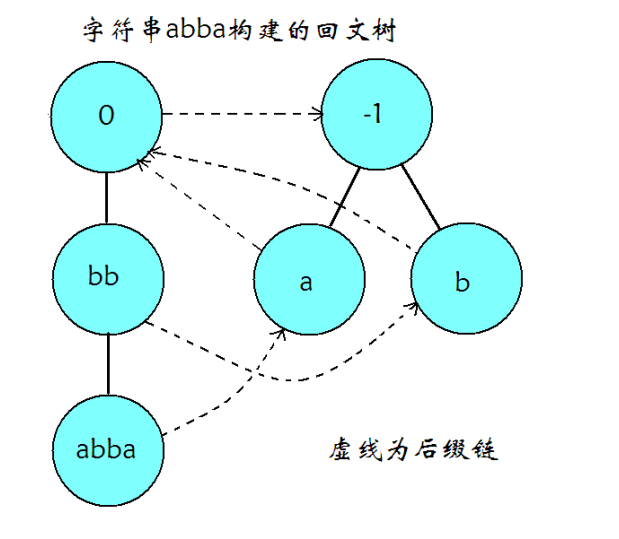
\includegraphics[width=.4\textwidth]{pic/pam1.png}
    \end{figure}
    \vspace{-1em}

    \pause PAM包含两棵树,一棵树中的节点对应的回文子串长度均为奇数,另一棵树中的节点对应的回文子串长度均为偶数。

    \pause 和其它的自动机一样,一个节点的 fail 指针指向的是这个节点所代表的回文串的最长回文后缀所对应的节点,但是转移边并非代表在原节点代表的回文串后加一个字符,而是表示在原节点代表的回文串前后各加一个相同的字符
\end{frame}

\begin{frame}[fragile]{建树}
    \small
    回文树有两个初始状态,分别代表长度为 -1,0 的回文串。我们可以称它们为奇根,偶根。它们不表示任何实际的字符串,仅作为初始状态存在。
    \vspace{1em}
    
    \pause 偶根的 fail 指针指向奇根,而我们并不关心奇根的 fail 指针,因为奇根不可能失配(奇根转移出的下一个状态长度为 1,即单个字符。一定是回文子串)

    \vspace{1em}
    \pause 类似SAM,我们一个一个字符添加,现在向自动机中添加\verb|S[k]|。

    \pause \vspace{1em}
    我们从以上一个字符结尾的最长回文子串对应的节点开始,不断沿着 fail 指针走,直到找到一个节点\verb|x|满足 \verb|S[k]==S[k-len[x]-1]|,即满足此节点所对应回文子串的上一个字符与待添加字符相同。
\end{frame}

\begin{frame}[fragile]{建树}
    \small
    现在,如果节点\verb|x|通过字母\verb|S[k]|的转移边已经被占用,我们无需做任何事情。否则我们要建一个新点\verb|q|。

    \pause \vspace{1em}
    显然新点的长度是\verb|len[x]+2|,它的 fail 指针?

    \pause \vspace{1em}
    找到 \verb|x| 在 fail 树上的某个尽量近的祖先 \verb|y|,使这个祖先前后加上\verb|S[k]|后能构成新点的回文后缀,也就是满足 \verb|S[k-len[y]-1]==S[k]|,那么令 \verb|fail[q]=ch[y][S[k]]|即可。
\end{frame}

\begin{frame}[fragile]{代码}
    \begin{minipage}{\linewidth}
    \begin{lstlisting}[language=c++]
int newnode(int x){len[++tot]=x;return tot;}
void pam_init(){tot=-1;newnode(0);newnode(-1);fail[0]=1;s[0]=-1;}
int find(int p){while(s[n]!=s[n-len[p]-1]) p=fail[p];return p;}
void insert(int c)
{
    s[++n]=c;
    int p=find(lst);
    if(!ch[p][c])
    {
        int q=newnode(len[p]+2);
        fail[q]=ch[find(fail[p])][c];
        ch[p][c]=q;
    }
    lst=ch[p][c];
}
    \end{lstlisting}
    \end{minipage}

    这是PAM的核心代码,很短。
\end{frame}

\begin{frame}{例题选讲:洛谷模板题}
给定一个字符串S,保证每个字符为小写字母。对于S的每个位置,请求出以该位置结尾的回文子串个数。

\vspace{1em}\pause
【题解】建PAM,维护节点深度,边建边输出当前点深度即可。
\end{frame}

\begin{frame}{例题选讲:[APIO2014] 回文串}
给你一个由小写拉丁字母组成的字符串S。我们定义S的一个子串的存在值为这个子串在S中出现的次数乘以这个子串的长度。
\vspace{1em}

对于给你的这个字符串S,求所有回文子串中的最大存在值

\vspace{1em}\pause
【题解】建PAM,如何求PAM中的节点所代表的回文串出现的次数?

\vspace{1em}\pause
每次插入完打一个+1标记,然后在fail树上自底向上累加即可。

\vspace{1em}\pause
题外话:PAM是2015年的科技,这是2014年的题,std的做法是manacher+SAM(或者manacher+SA),有兴趣可以看看
\end{frame}

\begin{frame}{例题选讲:CF835D}
\small
给定一个只包含小写字母的字符串$S$,对$k=1,...,|S|$,求有多少个$k$阶回文子串。一个串$T$是$k$阶回文串,需要满足:
\begin{itemize}
    \item $T$是回文串
    \item $T$的左半部分是$k-1$阶回文串(若$|T|$为奇数,则左半部分不包括中间)
\end{itemize}

原题数据范围只有$5000$,我们可以做的数据范围是$10^6$
\end{frame}

\begin{frame}[fragile]{例题选讲:CF835D}
\small
【题解】在PAM上维护一个\verb|g[x]|,指向\verb|x|的长度不超过\verb|len[x]/2|的最长回文后缀,维护方式类似fail:
\begin{lstlisting}[language=c++]
if(len[now]<=2) g[now]=fail[now];
else {
    int p=g[cur];
    while(s[n]!=s[n-len[p]-1]||(len[p]+2)*2>len[now]) p=fail[p];
    g[now]=ch[p][c];
}
\end{lstlisting}

\vspace{1em}\pause
接下来按转移图拓扑序dp即可(其实按点从小到大的顺序就行),设\verb|f[x]|表示节点\verb|x|最多是几阶回文,转移:\verb|f[x]=f[g[x]]+1|,然后统计答案输出即可。
\end{frame}

\begin{frame}[fragile]{例题选讲:[CERC2014] Virus synthesis}
\small
初始有一个空串,你每次可以在下面选一种操作执行:
\begin{itemize}
    \item 串开头或末尾加一个字符
    \item 串开头或末尾加一个该串的逆串
\end{itemize}

求构造$S$所需的最小操作次数,$|S|\leq 10^5$,字符集为\verb|{A,T,C,G}|
\end{frame}

\begin{frame}[fragile]{例题选讲:[CERC2014] Virus synthesis}
\small
【题解】建PAM,设\verb|f[x]|表示构造节点\verb|x|的串、且最后一步为复制,所需的最少操作数。(对于奇串无意义,因此为了方便,设奇串的\verb|f[x]=len[x]|)

\vspace{1em}\pause
若偶串\verb|z|(非空)可以通过加一个字母转移到\verb|x|,那么显然可以在\verb|z|复制之前添加一个字母,从而通过\verb|f[z]+1|次操作构造\verb|x|。因此为了方便,空偶串的\verb|f|值设为$1$

\vspace{1em}\pause
我们也可以找到长度不超过\verb|len[x]/2|的最长回文后缀,和上一题一样,就是\verb|g[x]|,然后通过\verb|g[x]|先填到\verb|x|的一半,然后做一次复制,操作次数是\verb|f[g[x]]+(len[x]/2-len[g[x]])+1|

\vspace{1em}\pause
结合上面两种转移,答案就是\verb|n-len[x]+f[x]|的最小值。
\end{frame}

\section{参考文献}

\begin{frame}[allowframebreaks]
    \bibliography{ref}
    \bibliographystyle{ieeetr}
    \nocite{*} % used here because no citation happens in slides
    % if there are too many try use:
    % \tiny\bibliographystyle{alpha}
\end{frame}


\begin{frame}
    \begin{center}
        {\Huge\calligra Thank You}
    \end{center}
\end{frame}

\end{document}